\documentclass[aspectratio=169,10pt,t]{beamer}
\usepackage{issa}  % place issa.sty in the same folder
\definecolor{AccentCol}{HTML}{A93226}
\renewcommand{\lecnum}{5}
\begin{document}
\titleslide{5}{Unsupervised Learning Part 2:\\Anomaly Detection \& Cybersecurity}{Statistical methods \textbullet\ Isolation Forest \textbullet\ One-Class SVM \textbullet\ Autoencoders \textbullet\ Intrusion detection \textbullet\ Insider threat\\Case A: network intrusion (N = 500K packets, 41 features) \textbullet\ Case B: insider threat (500 users, 15 compromised)}

\sect{1. Why Anomaly Detection}
\begin{frame}{Anomaly Detection --- Finding the Needle in the Haystack}
\begin{columns}[T]
\column{0.50\textwidth}
\begin{cbox}[ISSAnavy]{Clustering vs anomaly detection}\scriptsize \textbf{Clustering:} ``group similar things'' --- needs MOST data to form clusters; anomalies get forced into clusters or noise. \textbf{Anomaly detection:} ``learn what NORMAL looks like; flag everything that deviates''. NO attack labels needed $\Rightarrow$ catches \textbf{zero-day} threats never seen before.\end{cbox}
\begin{cbox}[ISSAgrn]{Defence relevance}\scriptsize Network intrusion detection $\bullet$ insider threat (credential compromise) $\bullet$ SIGINT anomalous transmission patterns $\bullet$ wargame and exercise data quality.\end{cbox}
\begin{cbox}{Learning objectives}\scriptsize\begin{te}\item Statistical outliers (z-score, Mahalanobis)\item Isolation Forest: path length $\to$ $O(1)$ inference\item One-Class SVM: $\nu$ and the RBF boundary\item Autoencoder reconstruction-error thresholds\item Apply all to intrusion and insider threat\item Evaluate TPR, FPR, AUROC at extreme imbalance\end{te}\end{cbox}
\column{0.48\textwidth}
\subhead{Three types of anomaly}
\figc{4.6cm}{\begin{tikzpicture}
\begin{scope}\draw[ISSAgrey](0,0)rectangle(4.6,1.4);\foreach \x/\y in {0.4/0.6,0.8/0.8,1.2/0.5,1.6/0.7,2.0/0.6,2.4/0.75,2.8/0.55,3.2/0.7,3.6/0.6,4.0/0.65}{\node[pt1]at(\x,\y){};}\node[pt2,inner sep=2pt]at(2.2,1.2){};\node[font=\scriptsize\bfseries,anchor=west]at(4.7,0.95){POINT};\node[lab,anchor=west,text width=2.6cm]at(4.7,0.45){one login at 3 a.m.\ from a foreign IP};\end{scope}
\begin{scope}[yshift=-1.8cm]\draw[ISSAgrey](0,0)rectangle(4.6,1.4);\draw[ISSAblue,thick,smooth]plot coordinates{(0.2,0.4)(0.7,1.0)(1.2,0.4)(1.7,1.0)(2.2,0.4)(2.7,1.0)(3.2,0.4)(3.7,1.0)(4.2,0.4)};\node[pt2,inner sep=2pt]at(2.45,0.95){};\node[font=\scriptsize\bfseries,anchor=west]at(4.7,0.95){CONTEXTUAL};\node[lab,anchor=west,text width=2.6cm]at(4.7,0.45){big transfer: normal on backup day, not at midnight Tuesday};\end{scope}
\begin{scope}[yshift=-3.6cm]\draw[ISSAgrey](0,0)rectangle(4.6,1.4);\foreach \x in {0.3,0.8,1.3,3.4,3.9,4.3}{\draw[ISSAblue](\x,0.2)--(\x,0.6);}\foreach \x in {1.8,1.9,2.0,2.1,2.2,2.3,2.4,2.5,2.6,2.7}{\draw[ISSAred,thick](\x,0.2)--(\x,0.6);}\node[font=\scriptsize\bfseries,anchor=west]at(4.7,0.95){COLLECTIVE};\node[lab,anchor=west,text width=2.6cm]at(4.7,0.45){each packet normal; 1,000 in 10 ms = port scan};\end{scope}
\end{tikzpicture}}
\end{columns}
\end{frame}

\begin{frame}{The Two Case Studies --- Network Intrusion and Insider Threat}
\begin{columns}[T]
\column{0.50\textwidth}
\begin{cbox}[ISSAred]{Case A --- network intrusion}\scriptsize 500,000 packet records (a 24-hour CERT log): \textbf{482,000 normal (96.4\%)}, \textbf{18,000 attacks (3.6\%)}. Attack types: DoS, Probe, R2L (remote-to-local), U2R (user-to-root). 41 packet features: duration, protocol, service, flag, source/destination bytes, wrong fragments, urgent, hot indicators, failed logins, guest login, connection count, SYN-error rate, REJ rate, \ldots\ Train 400,000 (normal + 14,400 attacks); test 100,000 (normal + 3,600 attacks).\end{cbox}
\figc{1.4cm}{\begin{tikzpicture}[x=0.135cm]\fill[ISSAblue!60](0,0)rectangle(96.4,0.5);\fill[ISSAred](96.4,0)rectangle(100,0.5);\node[white,font=\scriptsize\bfseries]at(48,0.25){normal 96.4\%};\node[font=\tiny,ISSAred,anchor=south]at(98.2,0.5){attack 3.6\%};\end{tikzpicture}}
\column{0.48\textwidth}
\begin{cbox}[AccentCol]{Case B --- insider threat}\scriptsize 500 users $\times$ 1,000 log entries = 500,000 activity logs. \textbf{Only 15 compromised accounts (0.003\%).} 18 behaviour features: login hour, login location (IP subnet), files accessed (count \& category), e-mail recipients (internal/external), USB/removable-drive events, after-hours flag, data-transfer volume, privilege-escalation attempts, failed authentications, app-usage deviation.\end{cbox}
\begin{wbox}\scriptsize Imbalance: Case A is 27 : 1; Case B is \textbf{33,333 : 1}. Accuracy is useless here: ``nothing is ever an attack'' scores 99.997\% on Case B.\end{wbox}
\end{columns}
\end{frame}

\sect{2. Statistical Methods}
\begin{frame}{Statistical Anomaly Detection (I) --- z-score and IQR Fences (Univariate)}
\begin{columns}[T]
\column{0.50\textwidth}
\figc{2.6cm}{\begin{tikzpicture}\begin{axis}[width=7.0cm,height=3.3cm,domain=-4.5:4.5,samples=80,ticks=none,xlabel={source bytes (z-score)},ymin=0]
\addplot[fill=ISSAblue!20,draw=ISSAblue,thick]{exp(-x^2/2)/2.5066}\closedcycle;
\draw[dashed,ISSAred](axis cs:-3,0)--(axis cs:-3,0.42);\draw[dashed,ISSAred](axis cs:3,0)--(axis cs:3,0.42);
\fill[ISSAamb](axis cs:-2.0,0.02)circle(2pt);\node[font=\tiny,anchor=south]at(axis cs:-2.0,0.06){DoS $z{=}-2.0$: missed};
\fill[ISSAred](axis cs:3.34,0.02)circle(2pt);\node[font=\tiny,ISSAred,anchor=south]at(axis cs:3.3,0.08){U2R $z{=}+3.34$};
\node[font=\tiny,ISSAred,anchor=south]at(axis cs:0,0.40){$\pm3\sigma$ fences};
\end{axis}\end{tikzpicture}}
\begin{fbx}{z-score}\[z_i=\frac{x_i-\mu}{\sigma},\qquad\text{anomaly if }|z_i|>\tau\ (\tau=2.5\text{ or }3)\]\end{fbx}
\begin{tl}\item Normal: $\mu=4{,}218$ B, $\sigma=2{,}104$ B; DoS avg 1.2 B $\Rightarrow z=-2.004$ (\textbf{missed} at $\tau=3$); U2R avg 11,240 B $\Rightarrow z=+3.34$ (\textbf{detected})\end{tl}
\column{0.48\textwidth}
\figc{1.5cm}{\begin{tikzpicture}[x=0.0009cm]\draw[ISSAgrey](0,0)--(8000,0);\fill[ISSAblue!30,draw=ISSAblue](2840,-0.25)rectangle(5620,0.25);\draw[ISSAblue,thick](4218,-0.25)--(4218,0.25);\draw[ISSAred,dashed](-1330,-0.4)--(-1330,0.4);\draw[ISSAred,dashed](9790,-0.4)--(9790,0.4);\node[font=\tiny,anchor=north]at(2840,-0.3){Q1 2,840};\node[font=\tiny,anchor=north]at(5620,-0.3){Q3 5,620};\node[font=\tiny,ISSAred,anchor=south]at(-1330,0.4){low fence $-1{,}330$};\node[font=\tiny,ISSAred,anchor=south]at(9790,0.4){high fence 9,790};\fill[ISSAamb](1.2,0)circle(2.5pt);\node[font=\tiny,anchor=south]at(400,0.3){DoS};\end{tikzpicture}}
\begin{fbx}{IQR fences (robust)}\[x<Q_1-1.5\,\text{IQR}\ \ \text{or}\ \ x>Q_3+1.5\,\text{IQR}\]\end{fbx}
\begin{tl}\item $Q_1=2{,}840$, $Q_3=5{,}620$, IQR $=2{,}780$ $\Rightarrow$ fences $-1{,}330$ and $9{,}790$\end{tl}
\begin{wbox}\scriptsize\textbf{Check the arithmetic:} the low fence is \emph{negative}, so DoS at 1.2 bytes lies \emph{inside} it and is not flagged. Univariate methods also see one feature at a time --- multi-feature attacks are invisible.\end{wbox}
\end{columns}
\end{frame}

\begin{frame}{Statistical Anomaly Detection (II) --- Mahalanobis Distance (Multivariate)}
\begin{columns}[T]
\column{0.48\textwidth}
\figc{2.7cm}{\begin{tikzpicture}[x=0.6cm,y=0.6cm]
\draw[ISSAgrey](-3.4,-2.4)rectangle(3.4,2.4);\foreach \x/\y in {-1.8/-1.0,-1.2/-0.8,-0.6/-0.3,0/0,0.6/0.3,1.2/0.7,1.8/1.0,-0.9/-0.7,0.9/0.5,-1.5/-0.6,1.5/0.9,0.3/0.3,-0.3/-0.2}{\node[pt1]at(\x,\y){};}
\draw[ISSAgrn,thick,rotate=30](0,0)ellipse(2.5 and 0.8);\draw[ISSAgrey,dashed](0,0)circle(1.9);
\node[pt2,inner sep=2pt]at(-1.0,1.1){};\node[font=\tiny,ISSAred,anchor=south]at(-1.0,1.2){outlier};
\node[lab,anchor=west]at(-3.3,-2.0){dashed: Euclidean circle (misses it)};\node[lab,ISSAgrn,anchor=west]at(0.4,-2.0){solid: Mahalanobis ellipse};
\end{tikzpicture}}
\begin{fbx}{Mahalanobis distance}\[D_M(x)=\sqrt{(x-\mu)^{\top}\Sigma^{-1}(x-\mu)}\]\end{fbx}
\begin{tl}\item Scales each direction by its variance and accounts for correlations ($\Sigma^{-1}$)\item $D_M^2\sim\chi^2_d$ under normality; threshold at 0.1\% FPR for $d=41$: $\approx9.46$\end{tl}
\column{0.50\textwidth}
\subhead{Mean $D_M$ by traffic type (threshold 9.46)}
\figc{2.6cm}{\begin{tikzpicture}\begin{axis}[ybar,width=6.8cm,height=3.3cm,symbolic x coords={Normal,Probe,R2L,DoS,U2R},xtick=data,ymin=0,ymax=21,bar width=13pt,nodes near coords,nodes near coords style={font=\fontsize{5.5}{6}\selectfont},ymajorgrids]
\addplot[fill=AccentCol!70]coordinates{(Normal,4.12)(Probe,7.24)(R2L,9.83)(DoS,12.41)(U2R,18.72)};
\draw[dashed,ISSAred,thick](axis cs:Normal,9.46)--(axis cs:U2R,9.46);
\end{axis}\end{tikzpicture}}
\begin{rbox}\scriptsize Overall test \textbf{TPR 72.1\%, FPR 1.8\%}. Probes (mean 7.24) fall below the threshold and are often missed; R2L is marginal.\end{rbox}
\begin{wbox}\scriptsize Assumes multivariate Gaussian data --- network traffic is heavy-tailed. \textbf{Robust variant:} estimate $\mu,\Sigma$ with the Minimum Covariance Determinant (central 50\% of data), so the anomalies don't contaminate $\Sigma$.\end{wbox}
\end{columns}
\end{frame}

\sect{3. Isolation Forest}
\begin{frame}{Isolation Forest --- Anomalies Are Easier to Isolate Than Normal Points}
\begin{columns}[T]
\column{0.52\textwidth}
\figc{2.8cm}{\begin{tikzpicture}[x=0.55cm,y=0.55cm]
\begin{scope}\draw[ISSAgrey](0,0)rectangle(5,4.4);\foreach \x/\y in {1.8/2.0,2.0/2.4,2.3/2.1,2.1/1.7,1.6/2.3,2.5/2.5,2.4/1.8,1.9/1.5}{\node[pt1]at(\x,\y){};}\node[pt2,inner sep=2pt]at(4.3,3.8){};
\draw[AccentCol,thick](3.6,0)--(3.6,4.4);\draw[AccentCol,thick](3.6,3.2)--(5,3.2);\node[font=\tiny,AccentCol]at(4.3,0.4){2 splits};\node[lab]at(2.5,-0.45){anomaly: isolated fast};\end{scope}
\begin{scope}[xshift=3.3cm]\draw[ISSAgrey](0,0)rectangle(5,4.4);\foreach \x/\y in {1.8/2.0,2.0/2.4,2.3/2.1,2.1/1.7,1.6/2.3,2.5/2.5,2.4/1.8,1.9/1.5}{\node[pt1]at(\x,\y){};}\node[pt3,inner sep=2pt]at(2.05,2.05){};
\foreach \a/\b/\c/\d in {3.0/0/3.0/4.4,0/2.9/3.0/2.9,1.2/0/1.2/2.9,1.2/1.3/3.0/1.3,2.6/1.3/2.6/2.9,1.2/2.2/2.6/2.2,1.95/1.3/1.95/2.2,1.95/1.9/2.6/1.9}{\draw[AccentCol](\a,\b)--(\c,\d);}\node[font=\tiny,AccentCol]at(4.0,0.4){8 splits};\node[lab]at(2.5,-0.45){normal point: many splits};\end{scope}
\end{tikzpicture}}
\begin{fbx}{Anomaly score}\[s(x,\psi)=2^{-E[h(x)]/c(\psi)},\quad c(\psi)=2H(\psi-1)-\tfrac{2(\psi-1)}{\psi}\]\end{fbx}
\sm{$h(x)$: path length from root to $x$; $E[h(x)]$: average over $B$ trees; $H(i)\approx\ln i+0.5772$. $s\to1$: anomaly; $s<0.5$: normal.}
\column{0.46\textwidth}
\begin{cbox}{Algorithm ($B=100$ iTrees)}\scriptsize For each tree: (1) sample $\psi=256$ points; (2) recursively pick a random feature $j$ and a random split $q\in[\min x_j,\max x_j]$; (3) stop when each leaf has one point or height reaches $\log_2\psi$. Shorter average path $\Rightarrow$ more anomalous.\end{cbox}
\begin{cbox}[ISSAgrn]{Why sub-sampling helps}\scriptsize With only 256 of 500K points per tree, normal points still sit among neighbours (many splits), while anomalies remain isolated (few splits): sub-sampling \emph{amplifies} the difference.\end{cbox}
\begin{rbox}\scriptsize\textbf{Case A ($B=100$, $\psi=256$):} TPR \textbf{91.4\%}, FPR 1.1\%, AUROC 0.976.\end{rbox}
\end{columns}
\end{frame}

\begin{frame}{Isolation Forest --- Computational Advantages and Path-Length Analysis}
\begin{columns}[T]
\column{0.48\textwidth}
\begin{fbx}{Cost}\[\text{train: }O(B\,\psi\log\psi)\qquad\text{infer: }O(B\log\psi)\]\end{fbx}
\begin{tl}\item $\log_2 256=8$ comparisons/tree $\times$ 100 trees = 800 comparisons per packet\item Training on Case A: \textbf{0.4 s} (vs 38.4 s for OCSVM); inference \textbf{0.002 ms}/packet --- real time\end{tl}
\subhead{Expected path length $E[h(x)]$ in 100 trees}
\figc{2.5cm}{\bars{8}{1.7}{1.0}{HTTP/6.84/ISSAblue,FTP/6.71/ISSAblue,DNS/7.12/ISSAblue,DoS/2.31/ISSAred,Probe/1.98/ISSAred,R2L/3.42/ISSAred,U2R/2.14/ISSAred}}
\column{0.50\textwidth}
\subhead{Anomaly score $s(x)$ (threshold 0.60)}
\figc{2.7cm}{\begin{tikzpicture}\begin{axis}[ybar,width=7.0cm,height=3.4cm,symbolic x coords={HTTP,FTP,DNS,DoS SYN,Port scan,Pwd brute,Root exploit},xtick=data,x tick label style={rotate=25,anchor=east,font=\fontsize{5}{6}\selectfont},ymin=0,ymax=1,bar width=10pt,nodes near coords,nodes near coords style={font=\fontsize{5}{6}\selectfont},ymajorgrids]
\addplot[fill=ISSAblue!60]coordinates{(HTTP,0.412)(FTP,0.422)(DNS,0.391)};\addplot[fill=AccentCol!80,bar shift=0pt]coordinates{(DoS SYN,0.861)(Port scan,0.887)(Pwd brute,0.742)(Root exploit,0.875)};
\draw[dashed,ISSAred,thick](axis cs:HTTP,0.6)--(axis cs:Root exploit,0.6);
\end{axis}\end{tikzpicture}}
\begin{ibox}\scriptsize\textbf{Why DoS has a short path:} its source bytes ($\approx$1) and connection count (thousands/s) are extreme, so the first random split on either feature isolates it immediately.\end{ibox}
\end{columns}
\end{frame}

\begin{frame}{Isolation Forest for SIGINT --- Zero-Day Detection of a New LPI Radar}
\begin{columns}[T]
\column{0.48\textwidth}
\begin{cbox}[ISSAnavy]{Normal SIGINT baseline (90 days)}\scriptsize Frequency 8.42 $\pm$ 0.12 GHz; PRF 1,240 $\pm$ 84 Hz; pulse width 2.1 $\pm$ 0.4 $\mu$s; scan rate 6.0 $\pm$ 0.8 deg/s.\end{cbox}
\figc{2.6cm}{\bars{1}{1.8}{1.7}{A: routine patrol radar/0.41/ISSAblue,B: known civilian ATC/0.38/ISSAblue,C: unusual PRF + freq./0.82/ISSAamb,D: never-seen LPI radar/0.91/ISSAred}}
\sm{Anomaly scores of four observed signals.}
\column{0.50\textwidth}
\begin{rbox}\scriptsize\textbf{Zero-day detection:} signal D was identified as a \textbf{Low-Probability-of-Intercept (LPI)} radar --- a new signature not in the threat library. No label was needed: its combination of frequency drift and random PRF was statistically unusual against the 90-day baseline.\end{rbox}
\begin{ibox}\scriptsize\textbf{Operational threshold selection:} choose $s^{*}$ to meet a target FPR $\le1\%$ on validation data, then report the TPR that results --- never tune the threshold on the test set.\end{ibox}
\begin{wbox}\scriptsize ``Unusual'' is not ``hostile'': signal C may be a new civilian system. Every alert needs analyst confirmation before the threat library is updated.\end{wbox}
\end{columns}
\end{frame}

\begin{frame}{The Recommended 3-Tier Hybrid Detection Architecture}
\figc{2.6cm}{\begin{tikzpicture}
\tikzset{T/.style={nd,text width=3.6cm,minimum height=1.7cm,font=\fontsize{6.8}{8}\selectfont}}
\node[ndN,minimum width=2cm,minimum height=1.7cm](in)at(0,0){all traffic\\\sm{$\sim$500K packets/day}};
\node[T,fill=ISSAblue!12,draw=ISSAblue](t1)at(3.6,0){\textbf{TIER 1 --- Isolation Forest}\\real-time screen, 0.002 ms\\flag if $s>0.55$};
\node[T,fill=AccentCol!12,draw=AccentCol](t2)at(8.0,0){\textbf{TIER 2 --- OCSVM / Autoencoder}\\deep scan of flagged packets only\\confirm or dismiss};
\node[T,fill=ISSAgrn!12,draw=ISSAgrn](t3)at(12.4,0){\textbf{TIER 3 --- Analyst}\\review high-confidence ($s>0.85$)\\update the threat library};
\draw[bigarr](in)--(t1);\draw[bigarr](t1)--node[above,font=\tiny]{small \% flagged}(t2);\draw[bigarr](t2)--node[above,font=\tiny]{confirmed}(t3);
\draw[arr,dashed](t3.south)--++(0,-0.4)-|node[pos=0.25,below,font=\tiny]{new signatures feed back into the baseline}(t1.south);
\end{tikzpicture}}
\begin{columns}[T]
\column{0.50\textwidth}
\begin{cbox}[ISSAnavy]{Why three tiers?}\scriptsize Tier 1 buys \textbf{speed} (screens everything), tier 2 buys \textbf{precision} (expensive models only where needed), tier 3 buys \textbf{knowledge} (humans confirm, explain and teach the system).\end{cbox}
\column{0.48\textwidth}
\begin{ibox}\scriptsize The same pattern is used in airport security (metal detector $\to$ scanner $\to$ officer) and in medical screening (cheap test $\to$ confirmatory test $\to$ specialist): cheap and sensitive first, expensive and specific second.\end{ibox}
\end{columns}
\end{frame}

\sect{4. One-Class SVM}
\begin{frame}{One-Class SVM --- A Tight Boundary Around Normal Data}
\begin{columns}[T]
\column{0.48\textwidth}
\figc{2.8cm}{\begin{tikzpicture}[x=0.6cm,y=0.6cm]
\draw[ISSAgrey](0,0)rectangle(7,4.6);\foreach \x/\y in {2.0/2.2,2.6/2.8,3.1/2.0,2.4/1.6,3.4/2.7,2.9/3.3,1.8/2.9,3.8/2.2,2.2/2.5,3.2/1.5}{\node[pt1]at(\x,\y){};}
\draw[AccentCol,thick,smooth cycle]plot coordinates{(1.3,2.4)(2.0,3.6)(3.2,3.8)(4.3,2.6)(3.6,1.0)(2.1,1.1)};
\foreach \x/\y in {5.8/3.9,0.6/0.6,6.0/1.0}{\node[pt2,inner sep=2pt]at(\x,\y){};}
\node[font=\tiny,AccentCol]at(3.0,4.2){$f(x)=0$};\node[lab]at(3.5,-0.4){trained on NORMAL data only};
\end{tikzpicture}}
\begin{fbx}{Sch\"olkopf (2001) formulation}\[\min\ \tfrac12\|w\|^{2}+\tfrac{1}{\nu N}\sum_i\xi_i-\rho\quad\text{s.t. }w\cdot\phi(x_i)\ge\rho-\xi_i\]\[f(x)=\text{sign}\Big(\sum_i\alpha_iK(x_i,x)-\rho\Big)\]\end{fbx}
\column{0.50\textwidth}
\begin{tl}\item $f(x)\ge0$: normal; $f(x)<0$: anomaly\item $\nu\in(0,1]$: \textbf{upper bound on the fraction of outliers}, lower bound on the fraction of support vectors; $\nu=0.01$ very tight; start with $\nu\approx$ target FPR\item RBF kernel $K=\exp(-\gamma\|x-x'\|^2)$: non-linear boundary in the original space\item \textbf{SVDD} alternative: minimum-radius hypersphere enclosing the data\end{tl}
\subhead{Grid search: TPR (\%) by $\nu\times\gamma$}
\figc{1.9cm}{\begin{tikzpicture}[x=1.15cm,y=0.42cm]
\foreach \ri/\nuv/\a/\b/\cc/\d in {0/0.01/71/81/87/74,1/0.05/79/88/89.7/79,2/0.10/82/89.1/86.3/72,3/0.20/84/86.4/78.2/64}{\node[font=\scriptsize\bfseries,anchor=east]at(-0.45,-\ri){$\nu{=}\nuv$};\foreach \ci/\v in {0/\a,1/\b,2/\cc,3/\d}{\pgfmathsetmacro{\pp}{(\v-60)*3}\node[fill=AccentCol!\pp!white,minimum width=1.1cm,minimum height=0.38cm,font=\scriptsize,inner sep=0.5pt]at(\ci,-\ri){\v};}}
\foreach \ci/\g in {0/0.001,1/0.01,2/0.10,3/1.0}{\node[font=\scriptsize\bfseries]at(\ci,0.75){$\gamma{=}\g$};}\draw[ISSAgrn,line width=1.3pt](1.55,-0.5)rectangle(2.45,-1.5);
\end{tikzpicture}}
\end{columns}
\end{frame}

\begin{frame}{One-Class SVM --- Case A Results and Limitations}
\begin{columns}[T]
\column{0.48\textwidth}
\begin{rbox}\scriptsize\textbf{Optimal $\nu=0.05$, $\gamma=0.10$:} test TPR \textbf{89.7\%}, FPR 0.9\%, AUROC 0.971. Training 38.4 s on 482K normal samples; inference 4.2 ms/packet.\end{rbox}
\figc{2.6cm}{\bars{40}{1.8}{2.0}{Isolation Forest train (s)/0.4/ISSAgrn,Autoencoder train (s)/12.8/ISSAblue,OCSVM train (s)/38.4/AccentCol}}
\column{0.50\textwidth}
\begin{wbox}\scriptsize\textbf{OCSVM limitations}\begin{tl}\item Training scales as $O(N^2)$: $482\text{K}^2$ is infeasible $\Rightarrow$ sub-sample 50K normal packets (verified: 88.9\% TPR, close to full)\item Sensitive to $\gamma$: the wrong value flags everything or nothing\item Not naturally probabilistic --- a binary decision only\end{tl}\end{wbox}
\begin{ibox}\scriptsize Use OCSVM for medium datasets where you want a principled, label-free boundary; prefer autoencoders or Isolation Forest at scale.\end{ibox}
\end{columns}
\end{frame}

\sect{5. Autoencoders}
\begin{frame}{Autoencoders --- Compress, Reconstruct: High Error = Anomaly}
\begin{columns}[T]
\column{0.52\textwidth}
\figc{2.7cm}{\begin{tikzpicture}
\foreach \x/\h/\lbl in {0/2.4/41,1.3/1.8/32,2.6/1.0/16,3.9/1.8/32,5.2/2.4/41}{\fill[AccentCol!25,draw=AccentCol](\x-0.25,-\h/2)rectangle(\x+0.25,\h/2);\node[font=\tiny]at(\x,-\h/2-0.2){\lbl};}
\fill[AccentCol!60](2.35,-0.5)rectangle(2.85,0.5);
\foreach \a/\b/\ha/\hb in {0/1.3/2.4/1.8,1.3/2.6/1.8/1.0,2.6/3.9/1.0/1.8,3.9/5.2/1.8/2.4}{\draw[ISSAgrey](\a+0.25,\ha/2)--(\b-0.25,\hb/2);\draw[ISSAgrey](\a+0.25,-\ha/2)--(\b-0.25,-\hb/2);}
\node[font=\scriptsize]at(-0.6,0){$x$};\node[font=\scriptsize]at(5.85,0){$\hat x$};\node[lab]at(1.3,1.45){encoder};\node[lab]at(3.9,1.45){decoder};\node[lab]at(2.6,0.8){bottleneck $h$};
\end{tikzpicture}}
\begin{fbx}{Training and detection}\[h=f_{\text{enc}}(x),\quad\hat x=f_{\text{dec}}(h),\quad L(\theta)=\tfrac1N\sum_i\|x_i-\hat x_i\|^{2}\]\[\text{RE}(x)=\|x-\hat x\|^{2}\ \Rightarrow\ \text{anomaly if }\text{RE}(x)>\tau\]\end{fbx}
\column{0.46\textwidth}
\figc{2.5cm}{\begin{tikzpicture}\begin{axis}[width=6.4cm,height=3.2cm,xlabel={reconstruction error},ylabel={density},xmin=0,xmax=0.55,domain=0:0.55,samples=80,ticks=none,legend pos=north east]
\addplot[fill=ISSAblue!25,draw=ISSAblue]{exp(-((x-0.024)/0.018)^2/2)/0.018}\closedcycle;\addlegendentry{normal}
\addplot[fill=ISSAred!25,draw=ISSAred]{4*exp(-((x-0.37)/0.08)^2/2)/0.08}\closedcycle;\addlegendentry{attacks}
\draw[dashed,thick](axis cs:0.087,0)--(axis cs:0.087,22);\node[font=\tiny,anchor=west]at(axis cs:0.09,20){$\tau=0.087$};
\end{axis}\end{tikzpicture}}
\sm{Normal RE mean 0.024 (sd 0.018); attack REs 0.29--0.46 by type (schematic shapes).}
\begin{tl}\item Trained on \textbf{normal data only}: it learns to rebuild normal traffic well and anything else badly\item Case A: $41\to32\to16\to32\to41$; 3,968 weights; Adam, lr 0.001, 50 epochs, batch 512\end{tl}
\end{columns}
\end{frame}

\begin{frame}{Types of Autoencoder --- and the Case A Result}
\begin{columns}[T]
\column{0.50\textwidth}
\begin{cbox}[ISSAnavy]{Vanilla AE (used in Case A)}\scriptsize Encoder--decoder with MSE loss; deterministic bottleneck.\end{cbox}
\begin{cbox}[ISSAblue]{Variational AE (VAE)}\scriptsize Bottleneck is a distribution $\mathcal{N}(\mu,\sigma^2)$; loss = MSE + KL penalty; gives a probabilistic (log-likelihood) anomaly score; smoother reconstructions for images.\end{cbox}
\begin{cbox}[ISSAgrn]{Sparse AE}\scriptsize L1 penalty on activations forces neurons to specialise $\Rightarrow$ better features.\end{cbox}
\begin{cbox}[violet]{Deep convolutional / LSTM AE}\scriptsize 1-D CNN or LSTM encoders capture local and temporal packet-sequence patterns --- for sequential traffic and user behaviour (Case B).\end{cbox}
\column{0.48\textwidth}
\subhead{Case A: vanilla AE, latent dimension 16}
\figc{2.4cm}{\bars{100}{1.7}{1.9}{TPR (\%)/95.8/ISSAgrn,AUROC $\times$100/98.8/ISSAblue,FPR $\times$10 (\%)/6/ISSAred}}
\sm{TPR 95.8\%, FPR 0.6\%, AUROC 0.988 --- best of all methods. Training 12.8 s; inference 0.04 ms.}
\begin{ibox}\scriptsize Threshold $\tau=0.087$ chosen to give FPR $=0.6\%$ on validation data --- the false-alarm budget comes first, the detection rate follows.\end{ibox}
\end{columns}
\end{frame}

\sect{6. Case A Results}
\begin{frame}{Network Intrusion Detection --- Case A Head-to-Head on 500K Packets}
\figc{2.6cm}{\scriptsize\renewcommand{\arraystretch}{1.13}\begin{tabular}{lccccccl}\toprule\textbf{Method}&\textbf{TPR}&\textbf{FPR}&\textbf{AUROC}&\textbf{Train}&\textbf{Infer (ms)}&&\textbf{Key limitation}\\\midrule z-score ($\tau$=3)&58.2\%&2.4\%&0.821&0.1 s&$<$0.01&&univariate; misses multi-feature attacks\\IQR fences&61.7\%&2.8\%&0.834&0.1 s&$<$0.01&&no correlations\\Mahalanobis&72.1\%&1.8\%&0.912&2.4 s&0.03&&assumes Gaussian; heavy tails\\Isolation Forest&91.4\%&1.1\%&0.976&0.4 s&\textbf{0.002}&&threshold tuning; no probabilities\\One-Class SVM&89.7\%&0.9\%&0.971&38.4 s&4.2&&slow; not scalable to 500K\\\rowcolor{ISSAgrn!20}\textbf{Autoencoder}&\textbf{95.8\%}&\textbf{0.6\%}&\textbf{0.988}&12.8 s&0.04&&GPU for big networks; black box\\\bottomrule\end{tabular}}
\begin{columns}[T]
\column{0.50\textwidth}
\figc{2.6cm}{\begin{tikzpicture}\begin{axis}[width=7.0cm,height=3.3cm,xlabel={false-positive rate (\%)},ylabel={true-positive rate (\%)},xmin=0.3,xmax=3.1,ymin=50,ymax=100,ymajorgrids,xmajorgrids]
\addplot[only marks,mark=*,mark size=2pt,AccentCol]coordinates{(2.4,58.2)(2.8,61.7)(1.8,72.1)(1.1,91.4)(0.9,89.7)(0.6,95.8)};
\node[font=\tiny,anchor=west]at(axis cs:2.4,58.2){z};\node[font=\tiny,anchor=west]at(axis cs:2.8,61.7){IQR};\node[font=\tiny,anchor=west]at(axis cs:1.8,72.1){Mahal.};\node[font=\tiny,anchor=west]at(axis cs:1.12,91.4){IF};\node[font=\tiny,anchor=north]at(axis cs:0.9,89.2){OCSVM};\node[font=\tiny,ISSAgrn,anchor=south west]at(axis cs:0.6,95.8){AE};
\end{axis}\end{tikzpicture}}
\column{0.48\textwidth}
\begin{rbox}\scriptsize\textbf{Autoencoder wins on every metric; Isolation Forest is the speed champion} (0.002 ms, trains in 0.4 s). Deploy IF as the tier-1 screen and AE as the tier-2 deep scan.\end{rbox}
\begin{wbox}\scriptsize\textbf{Real-world note:} these are KDD-Cup-99 / NSL-KDD-style benchmark results. Real enterprise networks show 10--100$\times$ higher FPR from legitimate unusual traffic (backups, batch jobs, patching): re-tune thresholds operationally.\end{wbox}
\end{columns}
\end{frame}

\begin{frame}{Autoencoder Performance by Attack Type}
\begin{columns}[T]
\column{0.52\textwidth}
\figc{3.3cm}{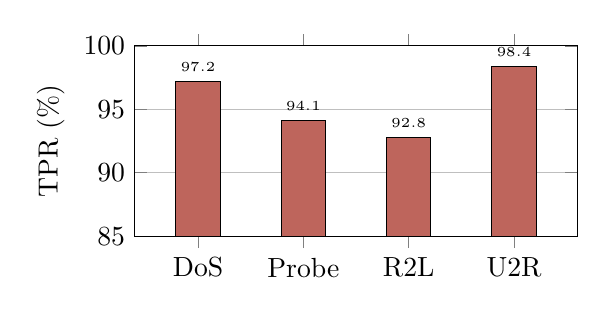
\begin{tikzpicture}\begin{axis}[ybar,width=7.2cm,height=4.0cm,symbolic x coords={DoS,Probe,R2L,U2R},xtick=data,ymin=85,ymax=100,bar width=16pt,nodes near coords,nodes near coords style={font=\fontsize{5.5}{6}\selectfont},ylabel={TPR (\%)},ymajorgrids,enlarge x limits=0.2]
\addplot[fill=AccentCol!75]coordinates{(DoS,97.2)(Probe,94.1)(R2L,92.8)(U2R,98.4)};
\end{axis}\end{tikzpicture}}
\sm{Attack counts: DoS 12,000; Probe 3,000; R2L 1,800; U2R 1,200.}
\column{0.46\textwidth}
\figc{2.3cm}{\bars{0.5}{1.6}{1.5}{DoS/0.412/AccentCol,Probe/0.318/AccentCol,R2L/0.291/AccentCol,U2R/0.461/AccentCol}}
\sm{Mean reconstruction error by attack type (normal mean = 0.024).}
\begin{ibox}\scriptsize\textbf{U2R} (user-to-root) is the hardest attack for statistical methods but the \emph{easiest} for the autoencoder: its feature combination is the most unlike anything in normal traffic. R2L, which imitates legitimate logins, is the hardest for the AE.\end{ibox}
\end{columns}
\end{frame}

\sect{7. Insider Threat}
\begin{frame}{Insider Threat (Case B) --- 15 Compromised Accounts in 500,000 Logs}
\begin{columns}[T]
\column{0.50\textwidth}
\begin{cbox}[ISSAred]{Extreme imbalance}\scriptsize 15 of 500,000 entries (0.003\%): \textbf{33,333$\times$} more normal than anomalous --- orders of magnitude more extreme than Case A (3.6\%).\end{cbox}
\begin{cbox}[ISSAnavy]{User behaviour analytics (UBA)}\scriptsize Instead of per-event detection, build a \textbf{behaviour profile per user}: login hour $\mu=9.4$ h, $\sigma=1.8$ h; 12--45 files/day; $<50$ MB/day transfer; 3--8 unique e-mail recipients/day. Anomaly = deviation from one's \emph{own} baseline. Sequence level: an LSTM autoencoder on 50-event sequences.\end{cbox}
\column{0.48\textwidth}
\figc{3.0cm}{\begin{tikzpicture}\begin{axis}[width=6.6cm,height=3.6cm,xlabel={login hour},ylabel={user X's login frequency},xmin=0,xmax=24,xtick={0,3,6,9,12,15,18,21,24},ymin=0,domain=0:24,samples=80,ticks=both,yticklabels={}]
\addplot[fill=ISSAblue!25,draw=ISSAblue]{exp(-((x-9.4)/1.8)^2/2)}\closedcycle;
\draw[ISSAred,thick](axis cs:2.28,0)--(axis cs:2.28,0.7);\fill[ISSAred](axis cs:2.28,0.7)circle(2pt);\node[font=\tiny,ISSAred,anchor=west]at(axis cs:2.6,0.75){02:17 Saturday $\Rightarrow$ $z\approx-4$};
\end{axis}\end{tikzpicture}}
\sm{User X normally logs in 9--11 a.m., never at weekends. A 02:17 Saturday login is about four standard deviations from X's own pattern.}
\end{columns}
\end{frame}

\begin{frame}{Insider Threat --- LSTM Autoencoder Results}
\begin{columns}[T]
\column{0.50\textwidth}
\begin{cbox}[ISSAnavy]{Architecture}\scriptsize Input: 50 events $\times$ 18 features. Encoder LSTM(64) $\to$ LSTM(32) $\to$ dense(16); decoder dense(32) $\to$ LSTM(64) $\to$ output. Trained on 475 non-compromised users. Per-user rolling RE (7-day window): normal baseline $0.031\pm0.014$; threshold $\tau=0.031+3(0.014)=\mathbf{0.073}$.\end{cbox}
\figc{2.2cm}{\bars{15}{1.5}{2.0}{Detected within 48 h/13/ISSAgrn,Missed/2/ISSAred,False alarms (30 days)/3/ISSAamb}}
\sm{13 of 15 = 86.7\% recall; 3 false alarms = 0.63\% of 475 users, cleared by analysts within 2 h.}
\column{0.48\textwidth}
\figc{2.2cm}{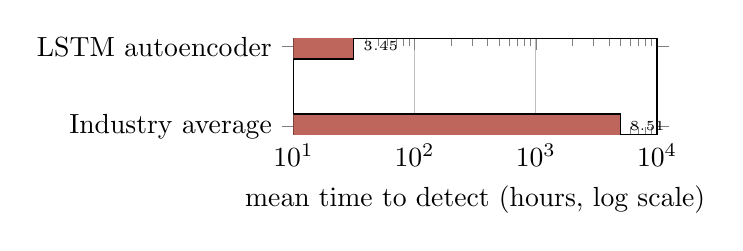
\begin{tikzpicture}\begin{axis}[xbar,width=6.2cm,height=2.8cm,symbolic y coords={Industry average,LSTM autoencoder},ytick=data,xmode=log,xmin=10,xmax=10000,xlabel={mean time to detect (hours, log scale)},bar width=9pt,nodes near coords,nodes near coords style={font=\fontsize{5.5}{6}\selectfont},xmajorgrids]
\addplot[fill=AccentCol!75]coordinates{(31.4,LSTM autoencoder)(4968,Industry average)};
\end{axis}\end{tikzpicture}}
\sm{MTTD 31.4 h vs an industry average of 207 days (4,968 h) for insider threats (IBM Cost of a Data Breach 2023).}
\begin{wbox}\scriptsize\textbf{The 2 missed accounts:} senior analysts whose legitimate weekend work was already in their baseline; attackers used the stolen credentials during the victim's normal hours. \textbf{Mitigation:} add data-access-category features --- no analyst should touch finance + HR + technical files in one session.\end{wbox}
\end{columns}
\end{frame}

\sect{8. Graph Anomalies}
\begin{frame}{Lateral Movement Detection --- Graph-Based Anomalies}
\begin{columns}[T]
\column{0.50\textwidth}
\figc{3.0cm}{\begin{tikzpicture}
\tikzset{M/.style={circle,draw=ISSAnavy,fill=ISSAlblue!50,minimum size=0.5cm,font=\tiny,inner sep=0pt}}
\node[M](w1)at(0,1.6){WS1};\node[M](w2)at(0,0.5){WS2};\node[M](w3)at(0,-0.6){WS3};\node[M,fill=ISSAred!40](w4)at(0,-1.7){WS4};
\node[M,minimum size=0.65cm](s1)at(2.4,1.0){SRV};\node[M,minimum size=0.65cm](s2)at(2.4,-0.8){FILE};\node[M,minimum size=0.75cm,fill=ISSAamb!50](dc)at(4.6,0.1){DC};
\foreach \u/\v in {w1/s1,w2/s1,w3/s2,w2/s2,s1/dc,w4/s2}{\draw[ISSAgrey,thick](\u)--(\v);}
\draw[ISSAred,very thick,dashed,->](w4)to[bend right=20]node[below,font=\tiny,ISSAred]{first-ever edge}(dc);
\node[lab]at(2.3,-2.5){$G_t=(V,E_t)$ vs 90-day baseline $G_{\text{base}}=(V,E_{\text{hist}})$};
\end{tikzpicture}}
\column{0.48\textwidth}
\begin{cbox}[ISSAnavy]{What is lateral movement?}\scriptsize After the initial compromise, the attacker moves through the network toward high-value targets (e.g.\ the domain controller). Signatures: unusual machine-to-machine connections (a first-time workstation $\to$ server link); SMB/RPC at odd hours; authentication from unexpected IPs; pass-the-hash (NTLM) patterns.\end{cbox}
\begin{rbox}\scriptsize\textbf{Anomaly signal:} a new edge $(u,v)$ in $G_t$ with no history in $G_{\text{base}}$ = high-suspicion event. Only 1.4\% of all connections are first-time, so the alert volume stays manageable.\end{rbox}
\end{columns}
\end{frame}

\begin{frame}{Graph Autoencoder for Command-and-Control (C2) Detection}
\begin{columns}[T]
\column{0.50\textwidth}
\begin{fbx}{Graph autoencoder}\[h=\text{GCN}(A,X),\qquad\tilde A=\sigma(hh^{\top})\]\[\text{node RE}_i=\big\|A_{i\cdot}-\tilde A_{i\cdot}\big\|^{2}\]\end{fbx}
\begin{tl}\item C2 malware beacons at near-constant inter-arrival times; JA3 = TLS fingerprint of the C2 client library\item Train the GAE on a 30-day normal network graph; compromised nodes' RE spikes when a C2 edge appears\end{tl}
\column{0.48\textwidth}
\subhead{25 simulated C2 channels, 10,000-node network}
\figc{2.2cm}{\bars{25}{1.5}{2.2}{Detected within 6 h/22/ISSAgrn,Missed (DGA)/3/ISSAred}}
\sm{88\% detected; 4.2 false positives per 10K nodes per day (FPR 0.042\%).}
\begin{wbox}\scriptsize\textbf{The 3 misses} used a domain-generation algorithm (DGA) with $>200$ randomised domains, avoiding a stable pattern. \textbf{Fix:} add a DNS feature such as DGA domain-name entropy.\end{wbox}
\end{columns}
\end{frame}

\sect{9. Comparison}
\begin{frame}{Algorithm Comparison --- Statistical $\to$ ML $\to$ Deep Learning}
\figc{3.0cm}{\scriptsize\renewcommand{\arraystretch}{1.12}\begin{tabular}{llcccccc}\toprule\textbf{Method}&\textbf{Type}&\textbf{TPR}&\textbf{FPR}&\textbf{AUROC}&\textbf{Train}&\textbf{Infer}&\textbf{Explainable}\\\midrule z-score / IQR&statistical&58--62\%&2.4--2.8\%&0.83&0.1 s&$<$0.01 ms&yes (intuitive)\\Mahalanobis&statistical&72.1\%&1.8\%&0.912&2.4 s&0.03 ms&yes (distance)\\Isolation Forest&ensemble&91.4\%&1.1\%&0.976&0.4 s&0.002 ms&partial (path)\\One-Class SVM&kernel ML&89.7\%&0.9\%&0.971&38 s*&4.2 ms&limited\\\rowcolor{ISSAgrn!20}Autoencoder&deep&95.8\%&0.6\%&0.988&12.8 s&0.04 ms&limited (RE)\\LSTM autoencoder&deep&86.7\%$^\dagger$&0.6\%&0.967$^\dagger$&48 s&0.8 ms&limited (RE)\\Graph AE&graph ML&88\%$^\dagger$&0.04\%&0.981$^\dagger$&varies&varies&partial\\\bottomrule\end{tabular}}
\sm{* needs sub-sampling for $N>50$K. $\dagger$ Case B insider / C2 metrics.}
\begin{columns}[T]
\column{0.50\textwidth}
\begin{rbox}\scriptsize\textbf{Accuracy winner:} autoencoder. \textbf{Speed winner:} Isolation Forest (0.002 ms/packet enables $\sim$1M packets/s screening). \textbf{Recommended:} 3-tier IF $\to$ AE $\to$ analyst.\end{rbox}
\column{0.48\textwidth}
\begin{wbox}\scriptsize\textbf{Explainability gap:} an RE value doesn't say WHY. For ROE compliance, apply SHAP to the reconstruction-error vector to show which features drove the alert.\end{wbox}
\end{columns}
\end{frame}

\sect{10. Across Disciplines}
\begin{frame}{Anomaly Detection Across the Disciplines}
\subhead{Spotting the abnormal is how engineers, doctors and watch-keepers stay alive}
\figc{5.0cm}{\begin{tikzpicture}
\tikzset{G/.style={nd,text width=4.75cm,align=left,minimum height=2.3cm,font=\fontsize{6.9}{8.2}\selectfont,inner sep=3pt}}
\node[G,draw=ISSAred,fill=ISSAred!6]at(-5,1.25){\textbf{\textcolor{ISSAred}{ENGINEERING}}\\Shewhart's control charts (Bell Labs, 1920s) flag a process as out of control when a measurement crosses $\pm3\sigma$ --- the z-score rule of this lecture.\\\textbf{Defence:} ammunition-lot quality assurance; production-line monitoring for weapons and spares.};
\node[G,draw=ISSAblue,fill=ISSAblue!7]at(0,1.25){\textbf{\textcolor{ISSAblue}{AERONAUTICS}}\\Engine health monitoring trends exhaust-gas temperature and vibration against each engine's own baseline to catch deterioration early.\\\textbf{Defence:} predictive maintenance of combat aircraft --- per-asset baselines, like UBA's per-user profiles.};
\node[G,draw=ISSAgrn,fill=ISSAgrn!7]at(5,1.25){\textbf{\textcolor{ISSAgrn}{BIOLOGY / MEDICINE}}\\The immune system separates ``self'' from ``non-self''; Forrest et al.\ (1994) turned this into artificial immune systems for computer intrusion detection.\\\textbf{Defence:} learn ``normal'' first; anything foreign is suspect --- the logic of Case A.};
\node[G,draw=violet,fill=violet!7]at(-5,-1.25){\textbf{\textcolor{violet}{PSYCHOLOGY}}\\Mackworth's clock test (1948), built to study RAF radar operators, showed detection accuracy falling sharply within the first half-hour of watch: the vigilance decrement.\\\textbf{Defence:} why automated tier-1 screening must support human analysts.};
\node[G,draw=ISSAamb,fill=ISSAyell!45]at(0,-1.25){\textbf{\textcolor{ISSAamb!80!black}{STATISTICS}}\\Benford's law: leading digits of many real datasets follow a fixed pattern, so fabricated numbers often stand out --- used in fraud and audit analytics.\\\textbf{Defence:} screening procurement claims and fabricated readiness or casualty reports.};
\node[G,draw=AccentCol,fill=AccentCol!8]at(5,-1.25){\textbf{\textcolor{AccentCol}{WARGAMING}}\\Anomaly scores on player and agent moves expose exploits, simulator bugs and ``gamey'' tactics that would never work in reality.\\\textbf{Use:} cleaner exercise data and more honest lessons learned.};
\end{tikzpicture}}
\begin{ibox}\scriptsize\textbf{Common thread:} define normal carefully, per asset or per person, and remember the base rate --- in every field, most alarms are false unless the threshold is set with care.\end{ibox}
\end{frame}

\sect{11. Summary}
\begin{frame}{Lecture 5 Summary --- Anomaly Detection for Defence Cybersecurity}
\figc{4.9cm}{\begin{tikzpicture}
\tikzset{K/.style={nd,text width=3.6cm,align=left,minimum height=2.1cm,font=\fontsize{6.4}{7.6}\selectfont,inner sep=3pt}}
\node[K,draw=ISSAblue,fill=ISSAblue!8]at(-4,1.2){\textbf{Z-SCORE \& MAHALANOBIS}\\Fast and interpretable; univariate z misses multi-feature attacks; Mahalanobis handles correlations but assumes Gaussian data.\\\textbf{Use:} quick baselines};
\node[K,draw=ISSAgrn,fill=ISSAgrn!8]at(0,1.2){\textbf{ISOLATION FOREST}\\Path-length score; 0.002 ms inference; zero-day detection without labels.\\\textbf{Use:} real-time tier-1 screening};
\node[K,draw=violet,fill=violet!8]at(4,1.2){\textbf{ONE-CLASS SVM}\\Tight boundary around normal; $\nu$ sets the outlier fraction; RBF kernel.\\\textbf{Use:} medium datasets, label-free};
\node[K,draw=AccentCol,fill=AccentCol!10,line width=1.2pt]at(-4,-1.2){\textbf{AUTOENCODER (DENSE / LSTM)}\\Reconstruction error = anomaly score; TPR 95.8\%, FPR 0.6\%; LSTM for behaviour sequences.\\\textbf{Use:} accuracy gold standard};
\node[K,draw=ISSAamb,fill=ISSAyell!40]at(0,-1.2){\textbf{GRAPH AE (C2 / LATERAL)}\\First-time edges and node RE expose lateral movement and C2; add DGA entropy for blind spots.\\\textbf{Use:} network graph intelligence};
\node[K,draw=ISSAred,fill=ISSAred!7]at(4,-1.2){\textbf{3-TIER DEPLOYMENT}\\IF screen $\to$ AE deep scan $\to$ analyst; insider MTTD 31.4 h vs 207 days.\\\textbf{Use:} operational best practice};
\end{tikzpicture}}
\end{frame}

\begin{frame}{Looking Ahead --- Lecture 6: Reinforcement Learning Part 1 --- Q-Learning \& MDPs}
\begin{columns}[T]
\column{0.50\textwidth}
\subhead{From passive learning to active decision-making}
\begin{tl}\item RL vs supervised / unsupervised\item MDP: $S$, $A$, $P(s'|s,a)$, $R(s,a,s')$, $\gamma$\item Bellman optimality: $V^*(s)$, $Q^*(s,a)$ derived from scratch\item Q-learning: TD update, $\varepsilon$-greedy, contraction-mapping convergence\item DQN: experience replay; target network; Double and Dueling DQN\item Reward shaping for sparse rewards; curriculum learning\end{tl}
\begin{ibox}\scriptsize\textbf{Assignment 5:} Isolation Forest path-length calculation + OCSVM $\nu$ interpretation + autoencoder threshold derivation.\end{ibox}
\column{0.48\textwidth}
\begin{cbox}{Preview: wargame tactical agent}\scriptsize $20\times20$ hex JANUS map; state space $\sim10^{28}$ (no Q-table can hold it); actions \{move N/S/E/W, attack, defend, resupply\}; reward $+10$ objective, $+5$ kill, $-8$ unit lost.\end{cbox}
\figc{2.3cm}{\bars{100}{1.6}{2.0}{Tabular Q (10$\times$10) vs random/91/ISSAgrn,DQN (20$\times$20) vs novice human/81/ISSAblue,DQN vs minimax AI/54/ISSAamb}}
\sm{DQN: 3 layers $\times$ 512 units; 100K-transition replay buffer; target update every 1,000 steps; 100K episodes, 48 GPU-hours.}
\end{columns}
\end{frame}
\end{document}
